\documentclass[article]{aaltoseries}
\usepackage[utf8]{inputenc}


\begin{document}
 
%=========================================================

\title{Implementing a Virtual Private Network System among Containers}

\author{Songlin Jiang% Your first and last name: do _not_ add your student number
\\\textnormal{\texttt{songlin.jiang@aalto.fi}}} % Your Aalto e-mail address

\affiliation{\textbf{Tutor}: Tuomas Aura} % First and last name of your tutor

\maketitle

%==========================================================

\begin{abstract}
This paper investigates the possibilities of implementing a Virtual Private Network (VPN) system among containers.

% TODO: Remove
More content to be added when this essay finishes.

\vspace{3mm}
\noindent KEYWORDS: Container, Network, Cloud, VPN

\end{abstract}


%============================================================


\section{Introduction}

In recent years, as an increasing number of applications have been moved to the cloud, container technologies such as Docker have received much attention from the industry and the academia. Containers are much more efficient and lightweight than virtual machines because containers share the Linux Kernel with the host. In contrast, virtual machines employ hardware virtualization and have their own instance of kernel, which needs more resources \cite{10.1145/2988336.2988337}.

VPNs are typically used in complex networking environments with many different network components. It is still a common practice \cite{9151942} to build and test network systems using virtual machines, which can be slow and troublesome. The problems can worsen when testing VPN systems, as each network component needs a virtual machine instance. It can be memory-consuming to simultaneously run multiple virtual machine instances on one host machine to simulate the network environment, which significantly perplexes testers with low-end devices and continuous integration and continuous delivery (CI/CD), as these environments are usually low on memory. Moreover, as Mac M1 / M2 chips are based on arm64 architecture, open-source virtual machine hypervisors are not currently well supported for arm64 hardware virtualization. However, arm64 is well supported by the containers \cite{9852232}.

Due to little research on implementing network systems using containers, this paper investigates the possibilities of implementing a VPN system based on Docker containers to overcome the disadvantages of virtual machines as mentioned above. This paper also analyze the functional and security limitations when implemented in this way.

This paper is organized as follows. Section 2 reviews the background of current technologies used for container networking and VPN systems. Section 3 defines our goal for implementing the VPN system using Docker containers, while Section 4 explains the details of our implementation. Section 5 presents our evaluation result by comparing the VPN system performance between the one implemented in the virtual machine and the one in the container. Finally, Section 6 provides the concluding remarks.

%============================================================


\section{Docker Networking System}
This section discusses the choice of the Docker container network driver for implementing the VPN system. It will also discuss how to enable routing and firewalls inside a container.

\subsection{Network Drivers}
Docker employs a pluggable networking subsystem. Several drivers can provide the docker network functionality, and the default ones include bridge, host, overlay, IPVLAN, MacVLAN, and none. We can choose one of them to implement the VPN system.

None, host, overlay drivers are not suitable for our scenario. Firstly, none driver disables all networking. Secondly, host driver is not necessary, as it can cause security implications due to its nature of sharing the same network stack with the host machine. In addition, overlay is not an appropriate option, as we are simulating the network system only on one host machine.

As a result, our possible candidates are bridge, IPVLAN, and MacVLAN. When looking into the details, bridge learns MAC addresses by looking into the frames headers of the communicating hosts. At the same time, the MacVLAN is a trivial bridge that does not need to learn as it already knows every MAC address it can receive. IPVLAN is very similar to MacVLAN, except that MacVLAN assigns a different MAC address to each attached docker container. In contrast, IPVLAN assigns the same MAC address to all containers attached to it.

Our final choice would be MacVLAN. As we will only use the driver to implement the internal network, there is no need to use advanced flood control and forwarding database manipulation that are specific to the bridge driver. Moreover, according to Docker's documentation related to networking \cite{docker_documentation_2023}, MacVLAN networks are the best choice when migrating from a VM setup, as MacVLAN makes the container appear as a physical device with its own MAC address. Besides, Gundall et al. \cite{9442123} conducts benchmarks for different virtualization technologies for networking overhead. The result shows that the MacVLAN driver has the best throughput while requiring the least CPU resources compared to other network drivers.

\subsection{Routing and Firewall}

Docker containers do not allow manipulating container network devices and setting routing tables or firewalls inside containers by default unless the net\_admin capability is assigned to the container.

According to capabilities man page \cite{capabilities}, assigning the net\_admin capability to containers allows performing the following network-related operations:
\begin{enumerate}
\setlength{\itemsep}{0pt}
\setlength{\parsep}{0pt}
\setlength{\parskip}{0pt}
\item Interface configuration;
\item Administration of IP firewall, masquerading, and accounting;
\item Modify routing tables;
\item Bind to any address for transparent proxying;
\item Set type-of-service (TOS);
\item Clear driver statistics;
\item Set promiscuous mode;
\item Enabling multicasting;
\item Use setsockopt(2) to set the following socket options:
SO\_DEBUG, SO\_MARK, SO\_PRIORITY (for a priority outside the
range 0 to 6), SO\_RCVBUFFORCE, and SO\_SNDBUFFORCE.
\end{enumerate}

As we are using the MacVLAN to build the internal network, all the network manipulations mentioned above only work for the network components that belong to the corresponding namespace. There should not exist any security implications to the host network if we give net\_admin capability to the container.

%\subsection{IPv6}

%============================================================


\section{Goal}

This paper simulates a scenario where the IoT devices (clients) in two sites A and B would like to connect to the server in the cloud S. The topology is based on the Aalto University CS-E4300 Network Security 2022-2023 instance Project 2 \cite{aura_peltonen_bui_2022}, where site A, site B and cloud S both use the private IP address to improve the security and save the IPv4 address. The gateway A, B and S connect the site A, site B and site S to the public Internet. The Router in the topology is a simplified version of Internet routers that routes across the Internet between the sites and the cloud. The address space between the gateway and the router simulates public, routable IPv4 addresses, even though it is actually private. site A, site B and cloud S all uses router to access the Internet.

In order to make the clients in both site A and site B connect to the cloud server safely, this paper uses strongSwan, a VPN implementation based on the Internet Protocol Security (IPsec).

We will try to implement two types of VPN: site-to-site and gateway-to-gateway.

\subsection{Site to Site}
\begin{figure}[t!]
  \begin{center}
    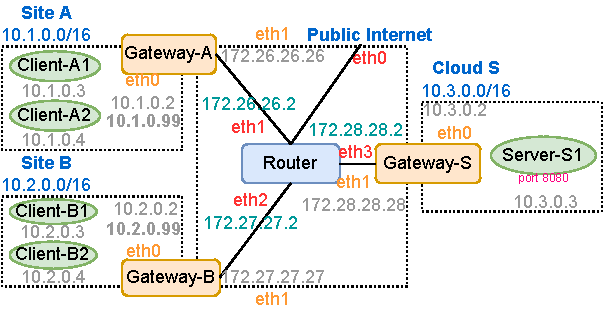
\includegraphics[width=1.1\textwidth]{figures/site-to-site.pdf}
    \caption{Site to Site}
    \label{fig:site2site}
  \end{center}
\end{figure}

A site-to-site VPN connects different network systems located at different sites together directly. In this case, the address space of the site A, B and Cloud S shouldn't overlap with each other.

Figure \ref{fig:site2site} shows the topology and corresponding address space under such circumstance.

\subsection{Gateway to Gateway}
\begin{figure}[t!]
  \begin{center}
    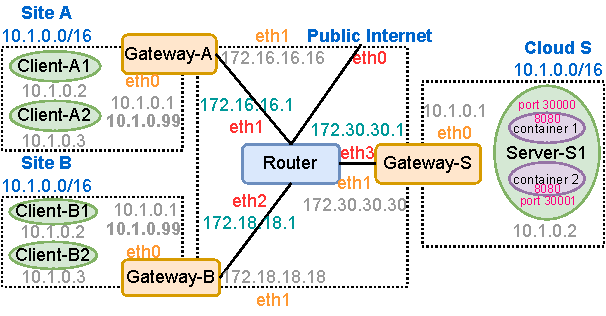
\includegraphics[width=1.1\textwidth]{figures/gateway-to-gateway.pdf}
    \caption{Gateway to Gateway}
    \label{fig:gateway2gateway}
  \end{center}
\end{figure}

A gateway-to-gateway VPN connects different gateways together. The packages then get routed to different clients within the corresponding site according to the routing table of the gateway.

Figure \ref{fig:gateway2gateway} shows the topology and corresponding address space under such circumstance.

%============================================================


\section{Implementation}



\subsection{Site to Site}

\subsection{Gateway to Gateway}

IP address spoofing

%============================================================


\section{Evaluation}

To be added.


%============================================================


\section{Conclusion}

To be added.


%============================================================


% \section{Simple things first}

% In this section, we give some simple examples of Latex mark-up.
% Sec.~\ref{sec:emphasis} emphasizes important points and
% Sec.~\ref{sec:math} gives examples of math formulas.
% Finally, \ref{sec:list} demonstrates lists.


% %------------------------------------------------------------


% \subsection{Emphasizing text}
% \label{sec:emphasis}

% \textit{Italics} is a good way to emphasize printed text. However,
% \textbf{boldface} looks better when converted to HTML.

% Paragraphs are separated by an empty line in the Latex source code.
% Latex puts extra space between sentences, which you must suppress
% after a period that does not end a sentence, e.g.\ after this acronym.

% Cross-references to figures (Fig.~\ref{fig:mypicture1}), tables
% (Table~\ref{tab:mytable1}), other sections (Sec.~\ref{sec:math})
% are easy to create. 


% %------------------------------------------------------------


% \subsection{Mathematics}
% \label{sec:math}

% In the mathematics mode, you can have subscripts such as $K_{master}$
% and superscripts like $2^x$. Longer formulas may be put on a separate
% line:
% \[ \emptyset \in \emptyset \; \Rightarrow \; E \neq mc^2. \]

% You may also want to number the formulas like Eq.~(\ref{eqn:myequation1})
% below.
% \begin{equation}\label{eqn:myequation1}
% C = E_{K_{public}}(P) = P^e. \hspace{10mm}   P = D_{K_{private}}(C) = C^d.
% \end{equation}



% %------------------------------------------------------------


% \subsection{Make a list}
% \label{sec:list}

% Lists can have either bullets or numbers on them. 

% \begin{itemize}
% \item one item
% \item another item, which is an exceptionally long one for an item
%   and consequently continues on the next line.
% \end{itemize}

% Lists can have several levels. Item~\ref{kukkuu} below contains
% another list.
% \begin{enumerate}
% \item the fist item \label{kukkuu}
%   \begin{enumerate}
%   \item the first subitem 
%   \item the second subitem
%   \end{enumerate}
% \item the second item
% \end{enumerate}


% %============================================================


% \section{More complex stuff}

% This section provides examples of more complex things.


% %------------------------------------------------------------


% \subsection{Data served on a table}


% Table~\ref{tab:mytable1} presents some data in tabular form. 

% \begin{table}[t!]
%   \begin{center}
%     \begin{tabular}{|l|lr|}
%     \hline
%     Protocol & Year &  RFC \\
%     \hline
%     TCP      & 1981 &  793 \\
%     ISAKMP   & 1998 & 2408 \\
%     Photuris & 1999 & 2522 \\
%     \hline
%     \end{tabular}
%     \caption{A table with some protocols}
%     \label{tab:mytable1}
%   \end{center}
% \end{table}


% %------------------------------------------------------------


% \subsection{Adding references}
% \label{sec:references}

% Do not forget to give pointers to the literature. If you are listing
% stuff related to your topic, you can give several references once
% \cite{Com00,HTS03,Nik99}. However, usually you should give only one, for example the standard describing the stuff \cite{RFC2408} and if you want to directly use someone else's words, use both quotation marks and refer to the source, for example that ``the developer does not need to know all about the framework to develop a working implementation'' \cite{Suo98}. Remember also to mark references to your pictures if they are not created by your own mind!

% If you plan to write with Latex regularly, create your own BibTeX
% database and use BibTeX to typeset the bibliographies automatically.
% In the long run, it will save you a lot of time and effort compared to
% compiling reference lists by hand.


% %------------------------------------------------------------


% \subsection{Embedded pictures}
% \label{sec:pictures}

% Fig.~\ref{fig:mypicture1} is an embedded picture. The supported formats for pictures
% depend on the actual LaTeX command used. For instance, regular \LaTeX supports
% pictures in EPS (Embedded PostScript) format, while pdf\LaTeX supports PDF (Portable
% Document Format), PNG (Portable Network Graphics) and JPEG (Joint Photographic Experts
% Group). It is recommended to use either EPS or PDF for diagrams as well as for any picture
% which includes vector images.

% \begin{figure}[t!]
%   \begin{center}
%     % Note how the file extension has been removed from the filename below
%     % so that the LaTeX command can automatically pick any supported file format
%     \includegraphics[width=.5\textwidth]{figures/sample}
%     \caption{An embedded picture}
%     \label{fig:mypicture1}
%   \end{center}
% \end{figure}


% %============================================================


% \section{Yet another section title}

% To be added.


%============================================================


\bibliographystyle{plain}
\bibliography{cs-seminar}

\end{document}
